\documentclass[tikz,border=8pt]{standalone}
\usepackage{tikz}
\usetikzlibrary{shapes,arrows,positioning}
\tikzstyle{proc}=[rectangle,draw,rounded corners,fill=blue!10,align=center,minimum width=3.4cm,minimum height=0.9cm,font=\small]
\tikzstyle{dec}=[diamond,draw,fill=green!10,align=center,aspect=2,font=\small]
\tikzstyle{term}=[rectangle,draw,rounded corners=8pt,fill=gray!15,align=center,minimum width=2.6cm,minimum height=0.9cm,font=\small\bfseries]
\tikzstyle{arr}=[->,thick]
\begin{document}
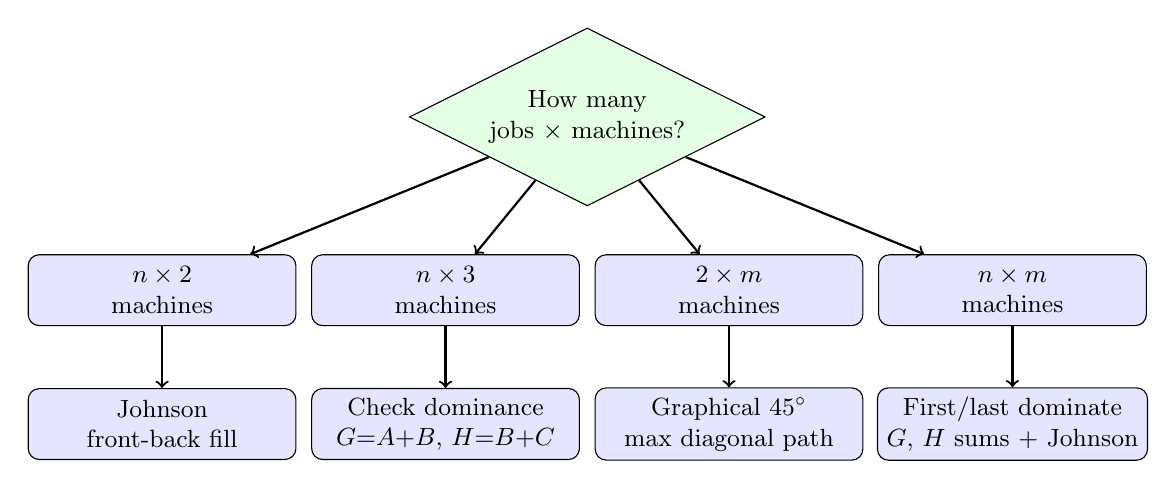
\begin{tikzpicture}[node distance=1.7cm]
\node[dec] (A) {How many\\jobs $\times$ machines?};
\node[proc, below of=A, xshift=-5.4cm, yshift=-0.5cm] (B) {$n\times 2$\\machines};
\node[proc, below of=A, xshift=-1.8cm, yshift=-0.5cm] (C) {$n\times 3$\\machines};
\node[proc, below of=A, xshift=1.8cm, yshift=-0.5cm] (D) {$2\times m$\\machines};
\node[proc, below of=A, xshift=5.4cm, yshift=-0.5cm] (E) {$n\times m$\\machines};
\node[proc, below of=B] (F) {Johnson\\front-back fill};
\node[proc, below of=C] (G) {Check dominance\\$G{=}A{+}B$, $H{=}B{+}C$};
\node[proc, below of=D] (H) {Graphical $45^\circ$\\max diagonal path};
\node[proc, below of=E] (I) {First/last dominate\\$G$, $H$ sums + Johnson};
\draw[arr] (A) -- (B);
\draw[arr] (A) -- (C);
\draw[arr] (A) -- (D);
\draw[arr] (A) -- (E);
\draw[arr] (B) -- (F);
\draw[arr] (C) -- (G);
\draw[arr] (D) -- (H);
\draw[arr] (E) -- (I);
\end{tikzpicture}
\end{document}
